\documentclass[11pt]{article}
\usepackage{graphicx} % Required for inserting images
\usepackage[natbibapa]{apacite}
\usepackage{natbib}
\usepackage{setspace}


\begin{document}
\begin{titlepage}
    \begin{center}
        \vspace*{1cm}
        
        \Large
        \textbf{Optimizing Model Selection in Microbial Growth Analysis: An Evaluation of Goodness-of-Fit Criteria and Statistical Approaches}
        
        \vspace{1.5cm}
        
        \textbf{Yutao ZHOU}\\
        Affiliation: Imperial College London\\
        Email: lz723@ic.ac.uk
        
        \vfill
        
        Word Count: 2673 words
        
        \vspace{0.8cm}
        
        \Large
        Date: 2 Dec 2023
        
    \end{center}
\end{titlepage}

\onehalfspacing
\section{Abstract}
Exploring the intricacies of microbial growth, this study delves into the comparative effectiveness of mechanistic and phenomenological models in predicting microbial behavior. The primary objective lies in assessing the suitability and precision of different models in encapsulating the dynamics of microbial growth rates. Methodologically, the research employs a combination of R-squared, Akaike Information Criterion (AIC), Bayesian Information Criterion (BIC), and Corrected Akaike Information Criterion (AICc) analyses to evaluate model performance. Results indicate a distinct superiority of logistic model in accurately depicting the growth patterns in bacterial cultures. The study reveals that simpler models like the phenomenological models provide baseline efficiency, but more complex models offer enhanced predictive accuracy in specific contexts. Conclusively, the research substantiates that models incorporating delay and stationary phases of growth, alongside traditional exponential parameters, yield more reliable predictions in complex microbial environments. This finding underscores the importance of model complexity in aligning with the biological realism of microbial growth, offering valuable insights for future research in microbial kinetics.
\section{Introduction}

Population dynamics play a crucial role in ecosystem functioning and characteristics such as carbon fixation rates and disease transmission\cite{Buchanan1997}\cite{Johnson2004}. Understanding population growth rates is vital in biology, as it helps in comprehending how populations respond to environmental pressures and reveals the intricacies of population-ecosystem interactions \cite{Levins1966}. According to the Malthusian principle, a population grows exponentially when its abundance is low, and resources are plentiful \cite{malthus1986essay}. However, this growth slows and eventually ceases as resources become limited \cite{Bolker2013}.

\hfill\break
Our study focuses on microbial (specifically, bacterial) growth rates. Bacterial growth in batch cultures follows distinct phases: lag, exponential, and stationary \cite{baranyi1994dynamic}. During the lag phase, bacteria activate transcriptional machinery, including genes involved in nutrient uptake and metabolic changes, preparing for growth \cite{Buchanan1997}. In the exponential phase, bacteria divide at a constant rate, with the population doubling each generation \cite{Motulsky2004}. Upon reaching the media's carrying capacity, growth slows, and the cell count stabilizes, marking the onset of the stationary phase \cite{Bolker2013}.

\hfill\break
In conventional methodologies, the quantification of microbial proliferation rates is accomplished by the graphical representation of cell counts or culture optical density as a function of time, utilizing a semi-logarithmic scale. This approach involves the delineation of a linear segment intersecting the phase of exponential growth, from which the maximal rate of growth can be extrapolated \cite{baranyi1994dynamic}. Subsequent advancements in this field have led to the formulation of more sophisticated models. These models are capable of encapsulating the entirety of the sigmoidal progression observed in bacterial growth patterns, thereby providing a more comprehensive understanding of the growth dynamics \cite{Motulsky2004}.


\subsection{Research Questions and Hypotheses}

This study aims to evaluate how well different mathematical models, such as those based on mechanistic theories of population growth versus phenomenological models, fit microbial population growth data across species. We hypothesize that mechanistic models, due to their biological foundations, might more accurately describe microbial growth processes, while phenomenological models, though flexible in handling complex data, might not accurately reflect biological realities \cite{Levins1966}\cite{Johnson2004}. By comparing the fit of these models, we aim to assess their strengths and limitations in practical applications. Additionally, we will explore modeling approaches to the time lag's impact on population growth and how different models address this aspect \cite{baranyi1994dynamic}\cite{Bolker2013}.

\hfill\break
Through this research, we hope to provide deeper insights into understanding and predicting microbial population dynamics, offering significant theoretical support for ecosystem management and biomedical research.

\section{Methods}

This section outlines the methodologies employed in the study, focusing on data collection, modeling approach, and the rationale behind the choice of computational tools.

\subsection{Data Preprocessing}

This study partitioned the dataset into 305 distinct subsets, each uniquely identified by combining several key attributes: species, growth medium, temperature, and the associated bibliographic reference. This stratification approach was instrumental in ensuring the analyses could account for variations attributable to these specific factors.

\hfill\break
After the initial segmentation, a crucial step in data preprocessing involved the creation of a new column, denoted as 'LogPopBio.' This column was generated by applying the natural logarithm transformation to the 'PopBio' data, which facilitates a more nuanced interpretation of population biology metrics by stabilizing variance and normalizing the data distribution.

\hfill\break
Further refinement of the dataset was undertaken by meticulously removing any records containing missing values (NA) across all subsets. This step was crucial to maintaining the subsequent analyses' integrity and reliability. Additionally, in alignment with the study's focus on growth dynamics, only those data points where the time was more significant than zero were retained for analysis. 

\subsection{Models}

In the scope of this research, a comprehensive analytical approach was employed, encompassing both linear and nonlinear modeling techniques. Specifically, the study incorporated three distinct linear models: a simple linear model, a quadratic polynomial model, and a cubic polynomial model. These models, which are phenomenological, were chosen for their ability to describe the data through varying degrees of polynomial relationships.

\hfill\break
Furthermore, the analysis extended to include two nonlinear models: the logistic growth model and the Gompertz model. These models were selected for their capacity to capture more complex, sigmoidal growth patterns typically observed in microbial population dynamics. The logistic model, renowned for its versatility in various biological contexts, is particularly adept at depicting population growth with a clear inflection point\cite{Agarwal}. Similarly, with its asymmetric sigmoidal curve, the Gompertz model offers a robust framework for modeling the initial lag phase followed by exponential growth and eventual stabilization\cite{Buchanan1997}.

\subsection{Model fitting}

Within the framework of this investigation, the R programming environment was utilized to execute both linear and nonlinear model fittings. To ascertain the initial estimates for the parameter maximum growth rate(Rmax) in nonlinear model fitting, a rolling regression methodology was implemented. This technique involved a systematic exploration of different window sizes, employing a trial-and-error approach to determine the optimal window size. It was observed that a window size of three yielded minimal errors in the fitting process, thereby enhancing the accuracy of the parameter estimation.

\hfill\break
The selection of appropriate models was underpinned by a comprehensive set of well-established criteria, primarily emphasizing goodness-of-fit measures. Among these measures, the coefficient of determination (R-squared) was utilized, offering insights into the proportion of variance in the dependent variable that can be explained by the independent variable(s). In addition to the conventional Akaike Information Criterion (AIC) and the Bayesian Information Criterion (BIC), the analysis was further enriched by incorporating the Corrected Akaike Information Criterion (AICc). The AICc is particularly valuable in scenarios where the sample size is small relative to the number of parameters, as it provides a more accurate estimation by adjusting for small sample sizes\cite{Johnson2004}. Moreover, the Akaike weights were employed as a probabilistic means of comparing models, offering a quantitative measure of the relative likelihood of each model given the data\cite{Wagenmakers2004}. Collectively, these criteria play a pivotal role in balancing model complexity and fit quality, thus guiding the selection of the most apt model for the data under examination.

\subsection{Computing language and Tools}
For data analysis and model fitting, this study predominantly employed the R programming language, a decision underpinned by its robust statistical computation capabilities and comprehensive suite of libraries tailored for nonlinear modeling. Notably, the nlsLM function from the minpack.The lm package was extensively utilized for its proficiency in handling nonlinear problems, most minor squares problems. Additionally, data visualization tasks were adeptly managed using the ggplot2 package, renowned for its versatility and ability to produce graphs of a quality suitable for publication.

\hfill\break
The analytical workflow was further enhanced by integrating several other R packages: readr for efficient data import, dplyr for data manipulation and transformation, and broom for converting statistical analysis objects into tidy data frames. The confluence of these packages provided a streamlined and efficient data processing pipeline.

\hfill\break
The rationale behind selecting R and its associated packages was predominantly dictated by their aptitude for managing complex datasets and conducting intricate statistical analyses. The comprehensive array of packages available within the R ecosystem facilitated a flexible approach to model fitting, catering to the diverse and specific needs of the study. Moreover, R's scripting nature aligns seamlessly with reproducible research principles, allowing for transparent and repeatable analyses. This attribute of R is particularly pivotal in scientific research, where reproducibility forms the cornerstone of empirical validation.

\section{Results}
\subsection{Model fitting}

In the course of fitting various models, it was observed that three distinct linear models exhibited satisfactory fitting characteristics. However, an anomaly was encountered with the logistic model, specifically at model 16, where an error impeded the fitting process. A subsequent adjustment of the window size parameter to 10 yielded a notable improvement in the model's fitting performance. Conversely, in the application of the Gompertz model fitting procedure, challenges were faced with models numbered 145, 178, 199, 213, 215, 244, 245, and 249, where the model failed to converge or fit the data appropriately. 

\subsection{$R^2$ AIC BIC and AICc values}
Following the completion of the model fitting process, we proceeded to calculate the R-squared (R²), Akaike Information Criterion (AIC), and Bayesian Information Criterion (BIC) values for each model. Subsequently, for two non-linear least squares (NLLS) models, the Corrected Akaike Information Criterion (AICc) was computed. To ensure the validity of our statistical analysis, values of negative infinity (-Inf) and positive infinity (Inf) within the AIC, BIC, and AICc datasets were systematically excluded. This exclusion was followed by the computation of the mean values for each of these metrics across all models. The results of these calculations were then systematically organized and presented in Table 1 for ease of interpretation and comparative analysis.
\hfill\break

 
 \begin{table}[ht]
     \centering
     \begin{tabular}{cccccc}
         Model & $R^2$ & AIC & BIC & AICc\\
         \hline
         & & & & \\
          Cubic & 0.8987831 & 10.890314 & 13.31370 &   \\
          Quadratic & 0.8443256 & 18.782590 & 20.60530 &   \\
          Linear & 0.6875294 & 32.365081 & 33.73211 &   \\
          Logistic & 0.9078786 & 6.253802 & 8.19251 & 11.15957 \\
          Gompertz & 0.8719611 & 10.183521 & 12.57910 & 19.01144 \\
          \hline
     \end{tabular}
     \caption{Mean of statistic value in each model type}
     \label{tab:my_label}
 \end{table}

\subsection{Best model in each subset}
In our analysis, we systematically identified the optimal model for each subset based on the criteria of highest R-squared, lowest Akaike Information Criterion (AIC), and lowest Bayesian Information Criterion (BIC) values. This methodical selection process aimed to ascertain the most statistically robust model for each respective subset. Subsequently, we quantified the frequency of each model type emerging as the best fit across all subsets. These frequencies were meticulously tabulated and presented in Table 2, providing a comprehensive overview of the model type predominance based on the aforementioned statistical parameters. This approach facilitates a nuanced understanding of the model efficacy in relation to the diverse dataset subsets.
\hfill\break
 \begin{table}[ht]
     \centering
     \begin{tabular}{cccccc}
         Model & $R^2$ & AIC & BIC \\
         \hline
         & & & & \\
          Cubic & 105 & 62 & 63   \\
          Quadratic & 5 & 25 & 24   \\
          Linear & 0 & 8 &  9  \\
          Logistic & 95 & 122 & 123 \\
          Gompertz & 98 & 86 & 84 \\
          \hline
     \end{tabular}
     \caption{Frequency of best model in 305 subsets}
     \label{tab:my_label}
 \end{table}

\subsection{Akaike Weight}
After conducting an in-depth analysis to ascertain the Akaike weights, the top ten models were identified as the most influential in our study. These models, which demonstrate the highest efficacy, are comprehensively listed in Table 3. To provide a visual representation of their performance, Figures 1 and 2 have been meticulously crafted. These figures offer a graphical depiction of the results, showcasing the attributes and behaviors of the selected models in a clear and accessible format.
\begin{table}[ht]
     \centering
     \begin{tabular}{cccccc}
         Model Number & ModelType & Akaike Weight  \\
         \hline
         & & & & \\
          3 & Linear & 4.177400e-01   \\
          3 & Quadratic & 2.547448e-01   \\
          3 & Logistic & 1.536783e-01  \\
          3 & Cubic & 9.966196e-02 \\
          3 & Gompertz & 7.343925e-02 \\
          4 & Linear & 2.201260e-04  \\
          4 & Quadratic & 1.924321e-04   \\
          4 & Gompertz & 1.467251e-04 \\
          4 & Cubic & 9.345684e-05 \\
          4 & Logistic & 8.125795e-05  \\
          \hline
     \end{tabular}
     \caption{Head 10 models with high Akaike weight}
     \label{tab:my_label}
 \end{table}
\begin{figure}[htbp]
    \centering
    \begin{minipage}{0.48\textwidth}
        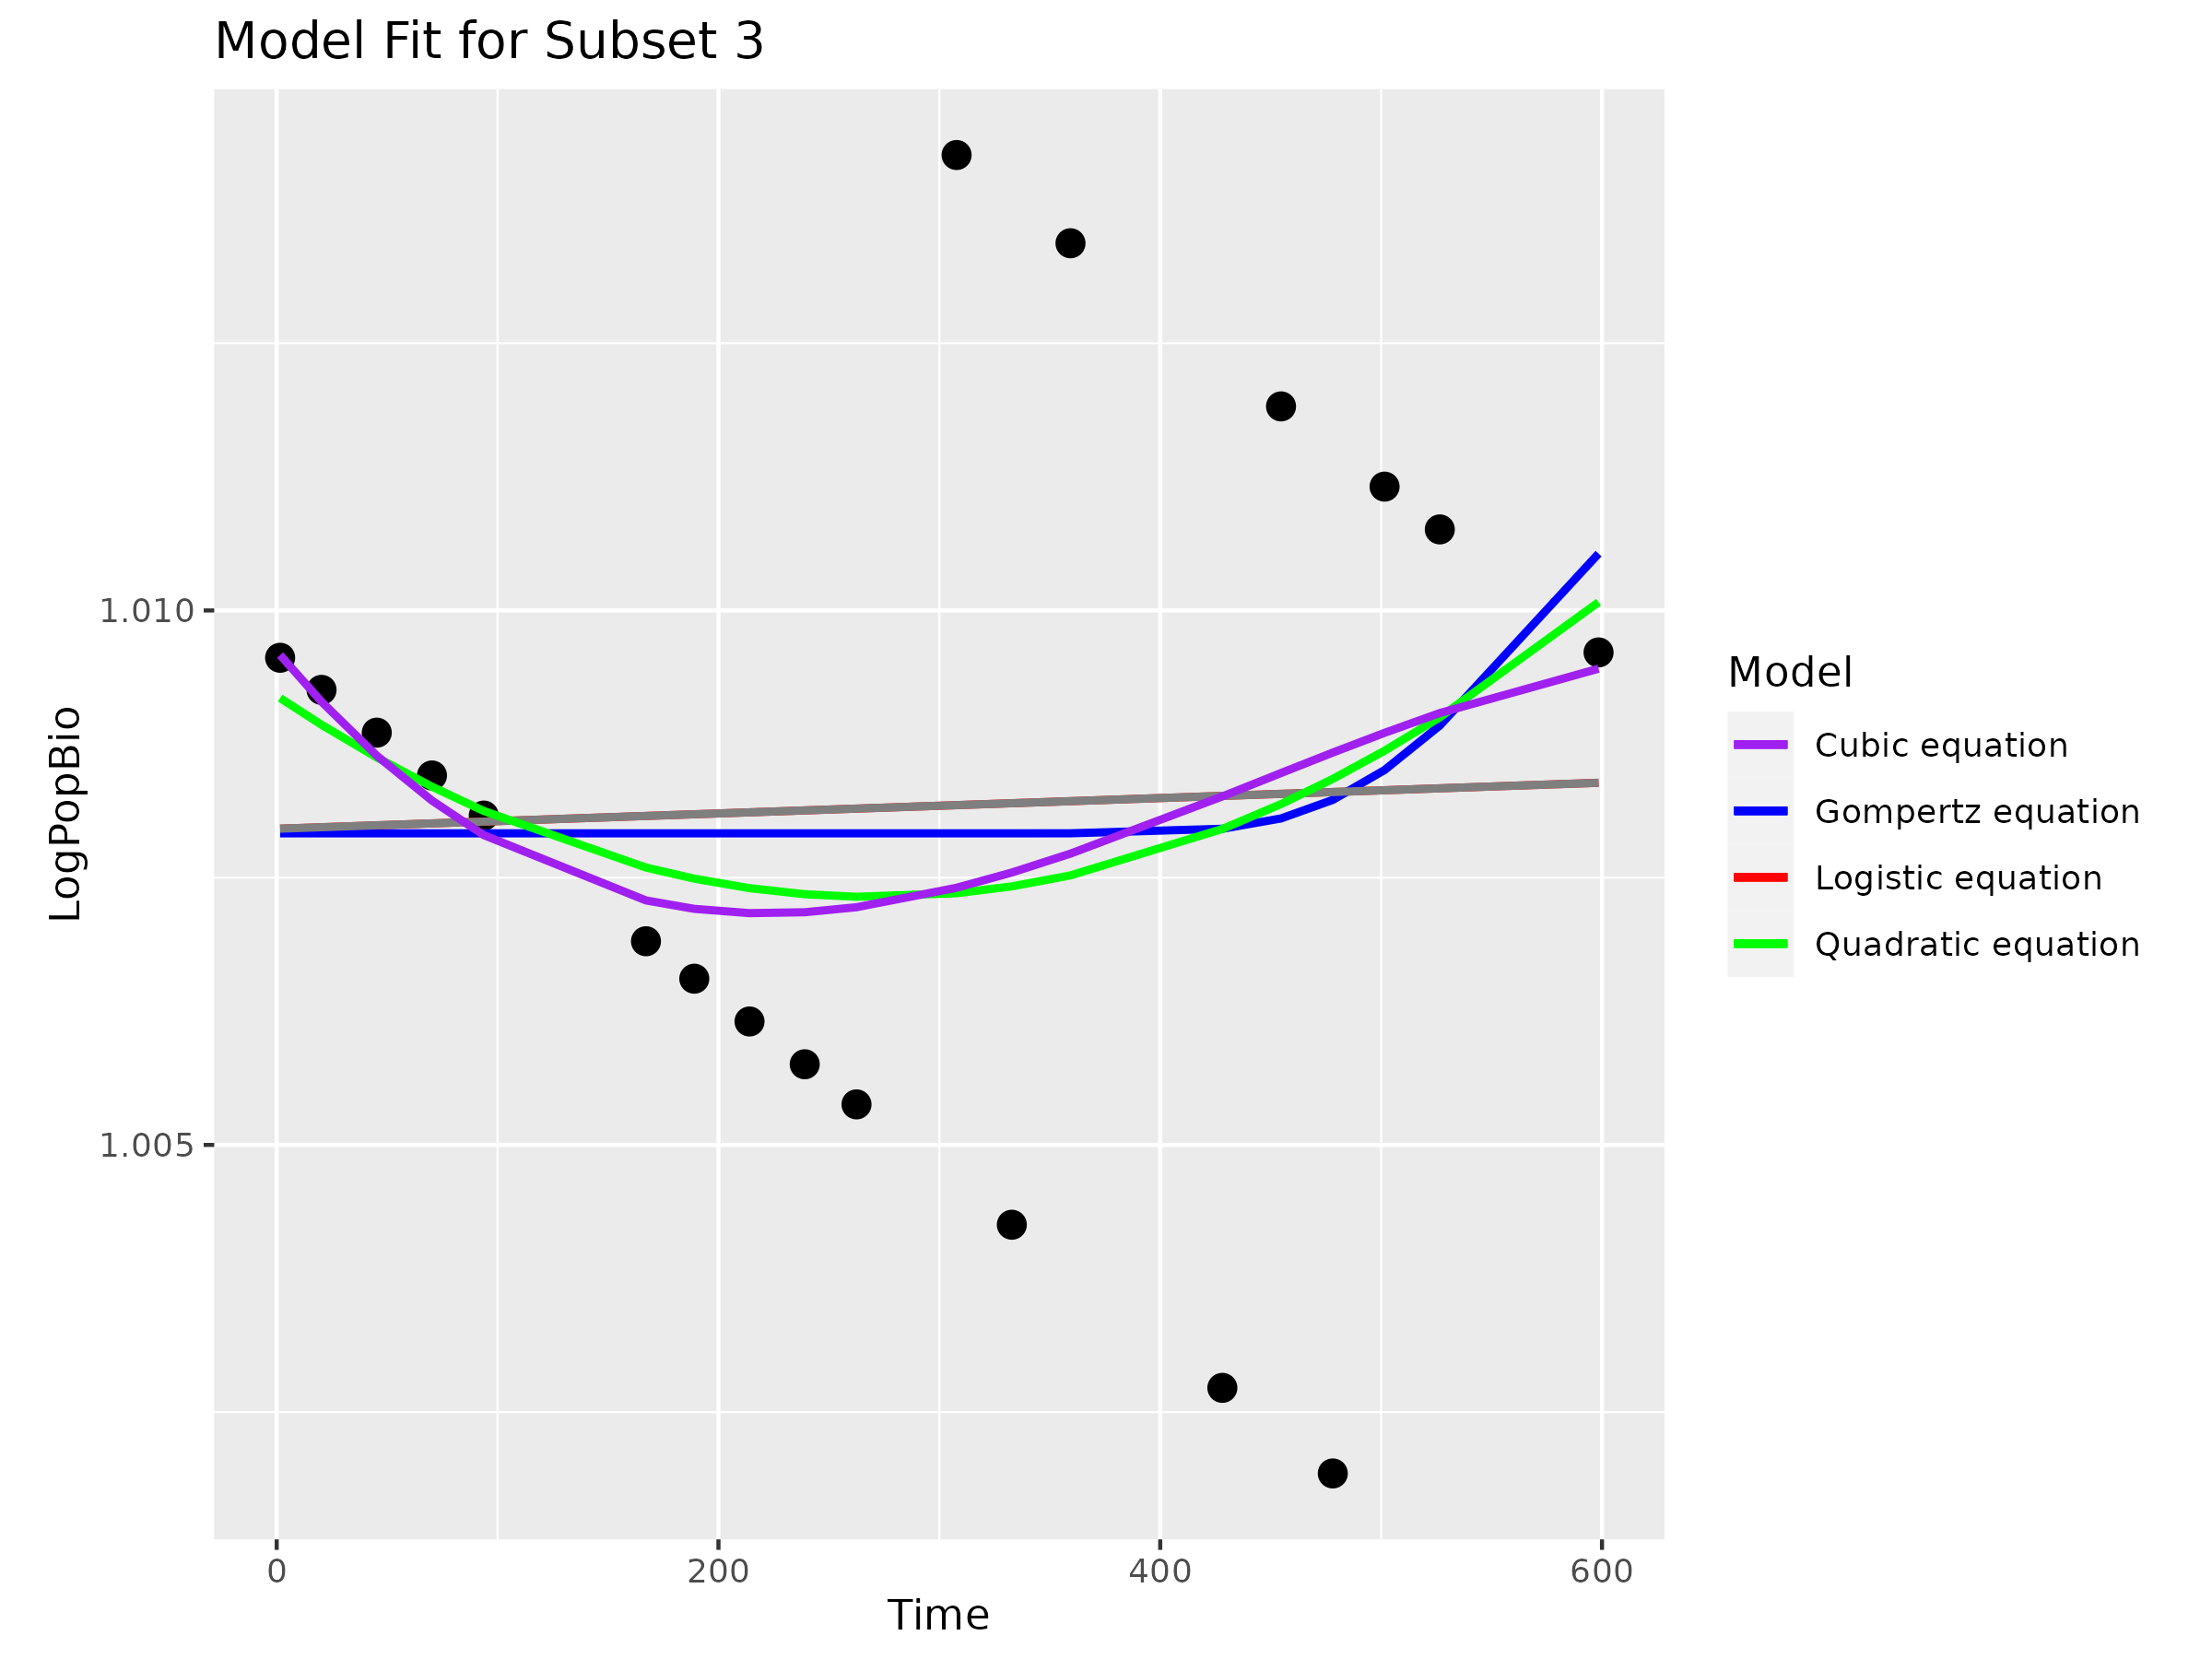
\includegraphics[width=\linewidth]{../results/plot/subset_3_plot.png}
        \caption{All models for subset 3}
        \label{fig:figure1}
    \end{minipage}\hfill
    \begin{minipage}{0.48\textwidth}
        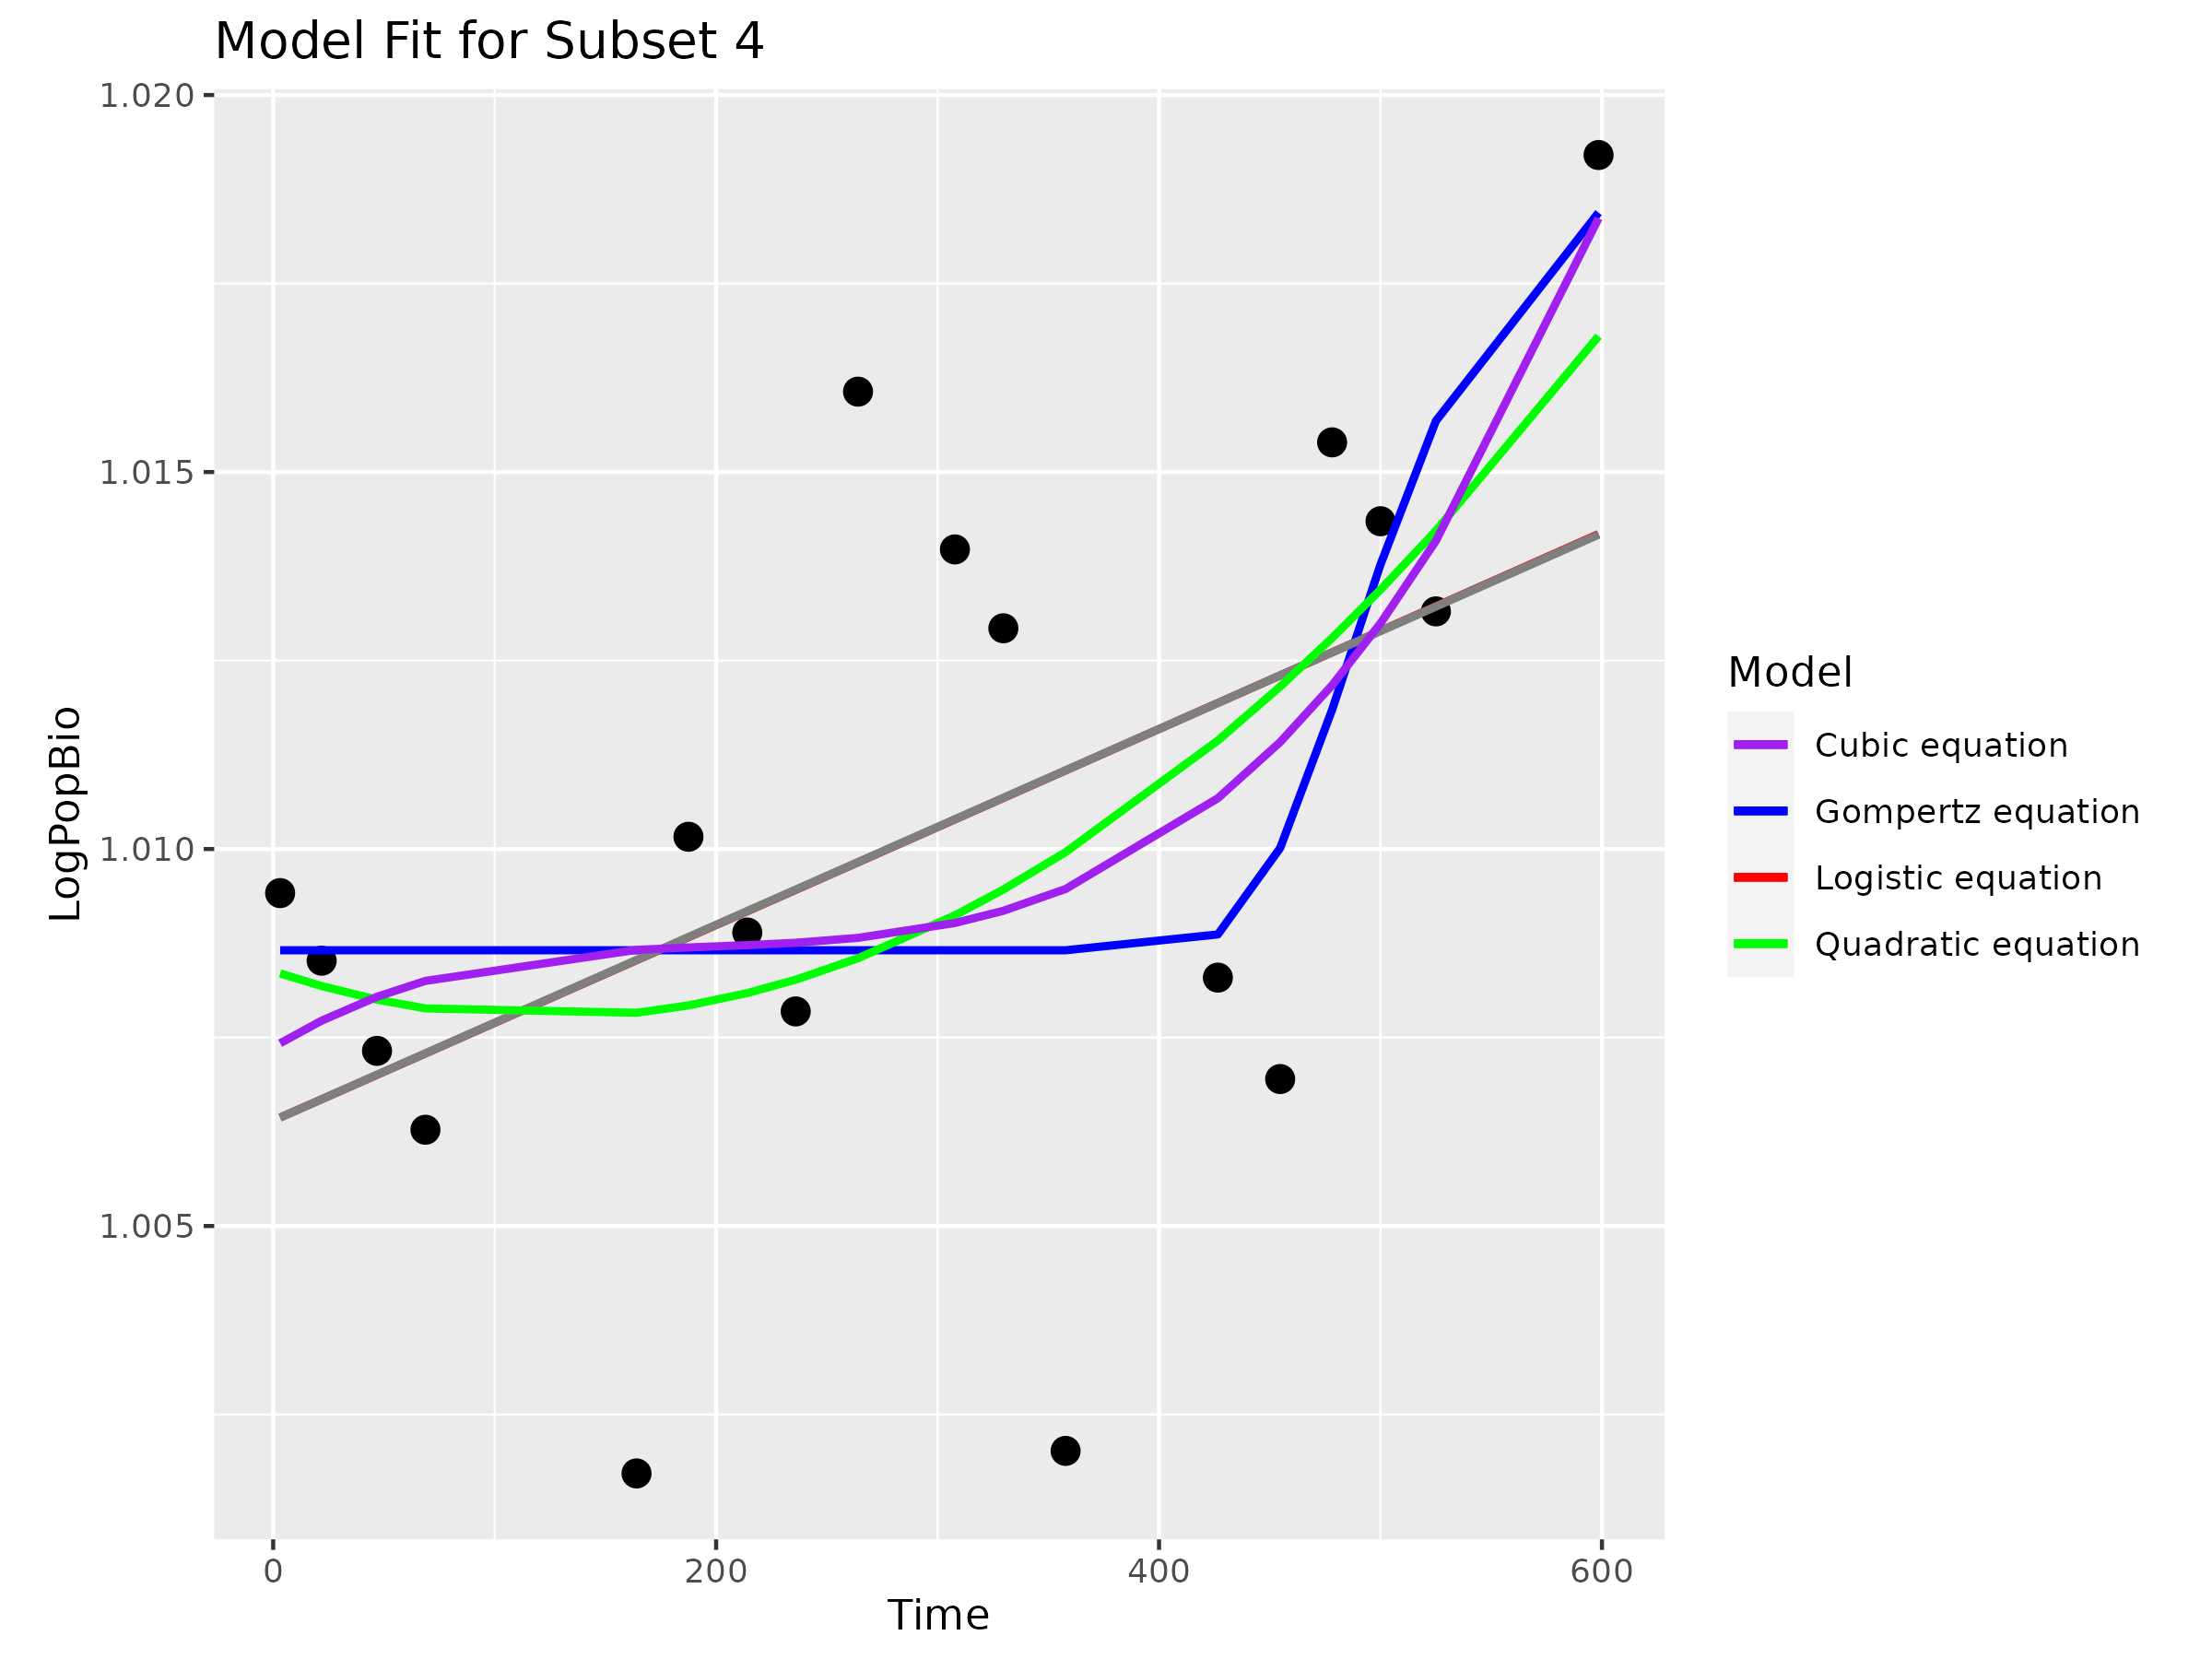
\includegraphics[width=\linewidth]{../results/plot/subset_4_plot.png}
        \caption{All models for subset 4}
        \label{fig:figure2}
    \end{minipage}
\end{figure}


\section{Discussion}
\subsection{Restatement of Objectives}
In addressing the research question, the study delved into various mathematical models to ascertain which best aligns with empirical microbial growth data across various species. A meticulous comparative analysis was conducted between mechanistic models grounded in biological theory and phenomenological models, with a focus on their descriptive efficacy.
\subsection{Summary of result finding}

Our investigation revealed that while phenomenological models, such as quadratic and cubic polynomials, exhibit a high degree of fit as evidenced by their respective \( R^2 \) values (0.8443256 for quadratic and 0.8987831 for cubic), the occurrence of infinite values in cubic fitting necessitates a cautious approach to their interpretive value. Although these models adeptly capture the complexity within the datasets, reflected in their AIC and BIC scores, they lack the biological interpretability offered by mechanistic models and may be prone to overfitting, as indicated by extreme values in some model fits.

\hfill\break
On the other hand, the logistic model, underpinned by biological principles, provided a robust fit with an \( R^2 \) value of 0.9078786 and furnished insights into the biological underpinnings of microbial population growth. This was complemented by the model's AIC and BIC values, which further substantiated its applicability. Despite certain instances of convergence issues, the Gompertz model remained a valuable contender, particularly for its representation of the lag phase in microbial growth.

\hfill\break
In addition, the analysis of model frequencies, as presented in Table 2, offers a comprehensive view of the comparative performance of each model across the 305 subsets. Notably, the cubic model demonstrated a predominant efficacy in frequency, emerging as the best fit in 105 subsets, an observation that, despite its tendency for overfitting, underscores its statistical robustness in a significant portion of the datasets. The logistic and Gompertz models also showed notable prevalence, being the best fit in 95 and 98 subsets, respectively, highlighting their relevance in capturing the growth dynamics of microbial populations. 

\hfill\break
In summary, the study underscores the logistic model's universality in depicting microbial growth across species while acknowledging the statistical significance and the nuanced data capture ability of quadratic and cubic models. The findings advocate a balanced approach to model selection that harmonizes the statistical robustness of phenomenological models with the biological relevance inherent in mechanistic models to enhance the predictability and understanding of microbial population dynamics.

\hfill\break
In addition, the analysis of model frequencies, as presented in Table 2, offers a comprehensive view of the comparative performance of each model across the 305 subsets. Notably, the cubic model demonstrated a predominant efficacy in terms of frequency, emerging as the best fit in 105 subsets, an observation that, despite its tendency for overfitting, underscores its statistical robustness in a significant portion of the datasets. The logistic and Gompertz models also showed notable prevalence, being the best fit in 95 and 98 subsets, respectively, which highlights their relevance in capturing the growth dynamics of microbial populations. 

\hfill\break
In summary, the study underscores the logistic model's universality in depicting microbial growth across species, while also acknowledging the statistical significance and the nuanced data capture ability of quadratic and cubic models. The findings advocate a balanced approach to model selection, one that harmonizes the statistical robustness of phenomenological models with the biological relevance inherent in mechanistic models, to enhance the predictability and understanding of microbial population dynamics.


\subsection{Contextualization Within the Wider Field}
In contextualizing our findings within the broader field of ecological modeling, this study contributes to an ongoing dialogue about the efficacy of different modeling approaches in understanding population dynamics. Notably, our results resonate with the findings of \cite{Johnson2004}, who emphasized the importance of model selection in accurately depicting ecological processes. Our study extends this conversation by specifically comparing the performance of mechanistic and phenomenological models in microbial growth, a topic also explored by \cite{Zwietering1990} in their examination of microbial ecology.

\hfill\break
Furthermore, the relevance of our study is highlighted by its alignment with the principles outlined by \cite{Graeme}, who advocate for integrating biological realism into ecological models. This approach is particularly pertinent given the growing recognition of the complexity of ecological systems, as discussed by \cite{Michael} in their exploration of ecosystem dynamics.

\hfill\break
By bridging these various perspectives, our research not only contributes to the theoretical understanding of microbial population dynamics but also offers practical insights for researchers and practitioners in the field of ecological modeling.

\subsection{Caveats and Future Directions}
\subsubsection{Error in Gompertz model fitting}
Despite the valuable insights garnered from this study, it is imperative to acknowledge certain limitations inherent in our research methodology. Specifically, the challenges encountered in fitting the Gompertz model underscore a critical need for enhanced precision in parameter estimation. This observation brings to light the complexities involved in accurately calibrating non-linear models, particularly when they are applied to diverse biological datasets. The Gompertz model, with its inherent intricacies, necessitates a sophisticated and nuanced approach to parameter estimation, which should ideally account for the biological context and the unique characteristics of each dataset. Addressing this limitation would not only improve the model's applicability but also augment the reliability and interpretability of the results in the context of microbial growth analysis. 

\subsubsection{Akaike weight selection}
Although the Akaike weight values for subsets 3 and 4 suggest a more effective overall model fitting, a closer examination of Figures 1 and 2 reveals that these particular subsets may not exemplify typical population growth patterns. This discrepancy raises critical questions regarding the limitations inherent in our analytical approach. Firstly, the Akaike weight, while a robust statistical measure, may not fully capture the biological nuances of population growth, particularly in cases where the data deviate from standard growth models\cite{Wagenmakers2004}. Secondly, the subsets in question could represent a typical or outlier growth scenarios that do not align well with the general trends observed in other datasets. This divergence could be attributed to unique environmental conditions, genetic variations in the microbial populations, or anomalies in data collection and recording. Lastly, the limitations of visual interpretation from Figures 1 and 2 should be considered. The graphical representation, while informative, might not accurately convey the complexities of the data, potentially leading to misinterpretations. Thus, a more comprehensive approach, incorporating both statistical rigor and biological context, is essential for a holistic understanding of microbial population dynamics.

\subsubsection{Other Limitations and Further Direction}
Moreover, the exclusion of environmental variables in our current modeling framework, predominantly executed within the R programming environment, opens up promising avenues for future research. This gap underscores the need to explore multi-variable models that integrate external environmental influences, as proposed by \cite{Micha2011}. While R is a powerful tool for statistical analysis, its application in this context may be limited by the availability of specialized packages that can effectively handle complex multi-variable ecological models. The integration of environmental variables could significantly enhance the explanatory power and predictive accuracy of the models. However, this advancement necessitates the development or refinement of R packages capable of managing the increased complexity and computational demands of such models. This approach aligns with the evolving paradigm in ecological modeling that advocates for a holistic perspective, considering both intrinsic biological factors and extrinsic environmental influences. Future research should also focus on overcoming the computational and methodological challenges inherent in extending the capabilities of R for more sophisticated ecological modeling.

\subsection{Conclusions}
In conclusion, while both mathematical and phenomenological models have their merits, the logistic model's consistent performance across diverse datasets underscores its utility in microbial growth modeling. Future research should aim to integrate adaptive algorithms for parameter estimation and consider the role of environmental variables to enhance the predictive power of growth models.


% References section

\newpage  
\bibliographystyle{apacite}
\bibliographystyle{apalike} 
\bibliography{miniproject.bib}

\end{document}